\documentclass[journal, a4paper]{IEEEtran}

\usepackage{graphicx}   
\usepackage{url}        
\usepackage{amsmath}    
\usepackage{hyperref}


% Your document starts here!
\begin{document}

% Define document title and author
	\title{Bitcoin Blockchain Visualization}
	\author{Zhiyi Xu, and Ruolan Zeng}
	\maketitle
                                                   
% Each section begins with a \section{title} command
\section{Introduction}
	% \PARstart{}{} creates a tall first letter for this first paragraph
	\PARstart {B}{lockchain} and bitcoin are both hot topics these days. Bitcoin is a distributed, decentralized crypto-currency. A blockchain is a distributed database that is used to maintain a continuously growing list of records, called blocks. Bitcoin uses the blockchain protocol to serialize transactions of the bitcoin currency among its users. Figure 1 is an image briefly introducing how blockchain works for bitcoin.
\begin{figure}[!hbt]
		\begin{center}
		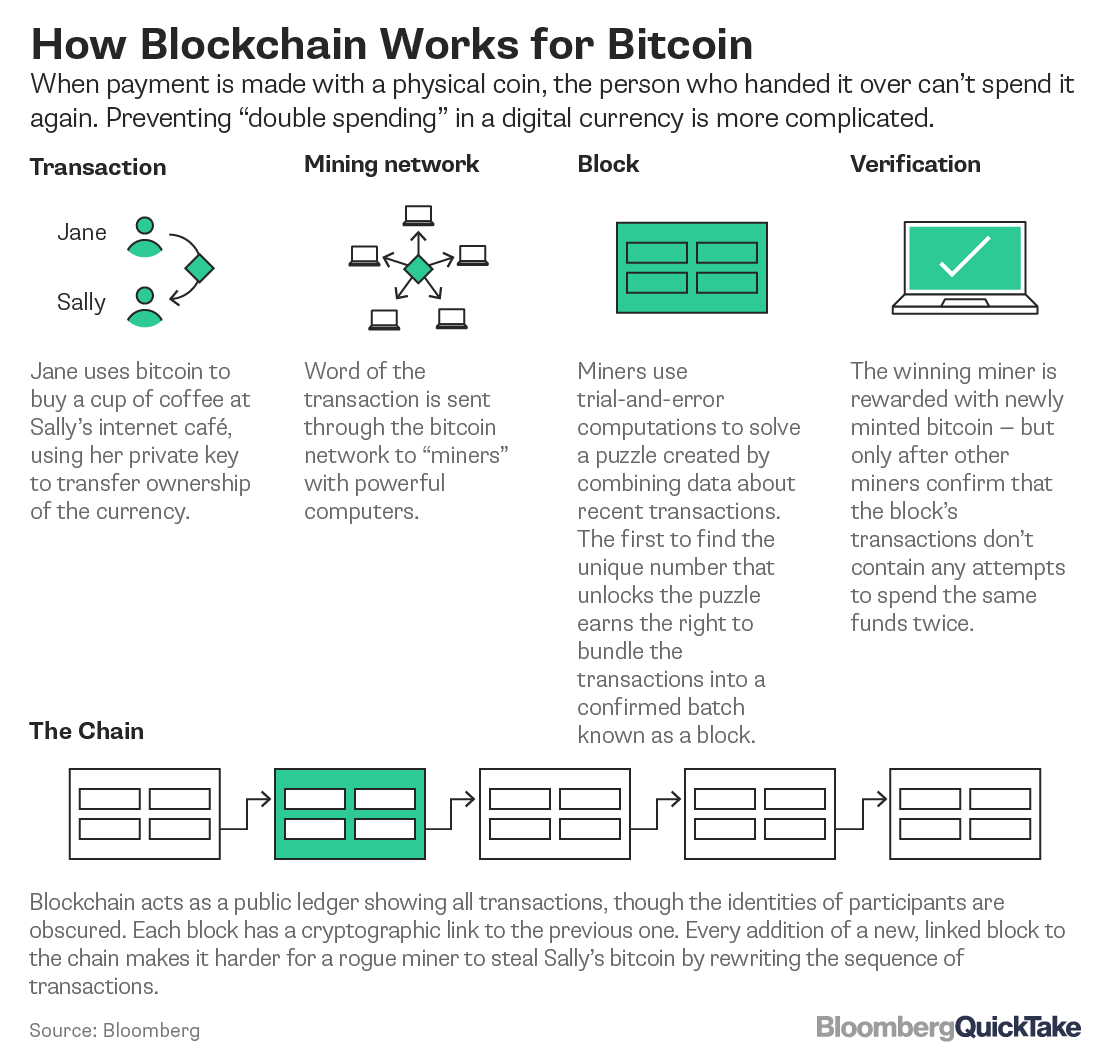
\includegraphics[width=\columnwidth]{how_blockchain_works.png}
		\caption{an image briefly introducing how blockchain works for bitcoin}
		\label{fig:how_blockchain_works}
		\end{center}
	\end{figure}

\section{Motivation}
Blockchain is a hot topic these days. Even though there are a huge number of video and blog tutorials for blockchain beginners on the internet, people are still asking "what is blockchain ?", meaning that blockchain could be a very abstract concept and takes a relatively longer time for people to understand. In this case, the use of visualization could be very helpful. So we want to do a learning project in which we mock and visualize the bitcoin blockchain. We aim to study the concept of bitcoin and blockchain thoroughly and deeply.

\section{Gap}
Since we want to build a visualization, the first and biggest challenge is the overall design of the visualization. Some existing visualizations focus on how transactions are generated and how them are added into blocks, then we'll lose an overall view of how the whole blockchain works. Other existing visualizations focus more on how blocks are added by miners and how blockchain is generated, then we'll lose a detailed view of transaction fees, why some transactions are recorded into the blocks while others are not. Other challenges would be how to get the data and how to design the data structure.

\section{Problem statement}
Design and build a bitcoin blockchain visualization that demonstrates both overall and detailed view of how bitcoin blockchain works, helping others to study the concept of bitcoin and blockchain thoroughly and deeply.

\section{Overall design}
Figure 2 is the initial state of the overall design of our bitcoin blockchain visualization.
\begin{itemize}
    \item Time slider: the time range within which transactions and blocks are generated. It can be used to choose the time point by dragging it to the point. You can also use the "Play" button to make it move automatically. And "Pause" it with the same button.
    \item Right panel: all the bitcoin addresses in the system and the transactions were made by those addresses. Nodes that have transactions happening between them will form subgraphs and be dragged closer.
    \item Left panel's upper layer: the blockchain
    \item Left panel's middle layer: detailed information of selected transaction
    \item Left panel's lower layer: all transactions happening at present time point
\end{itemize}

\begin{figure}[!hbt]
		\begin{center}
		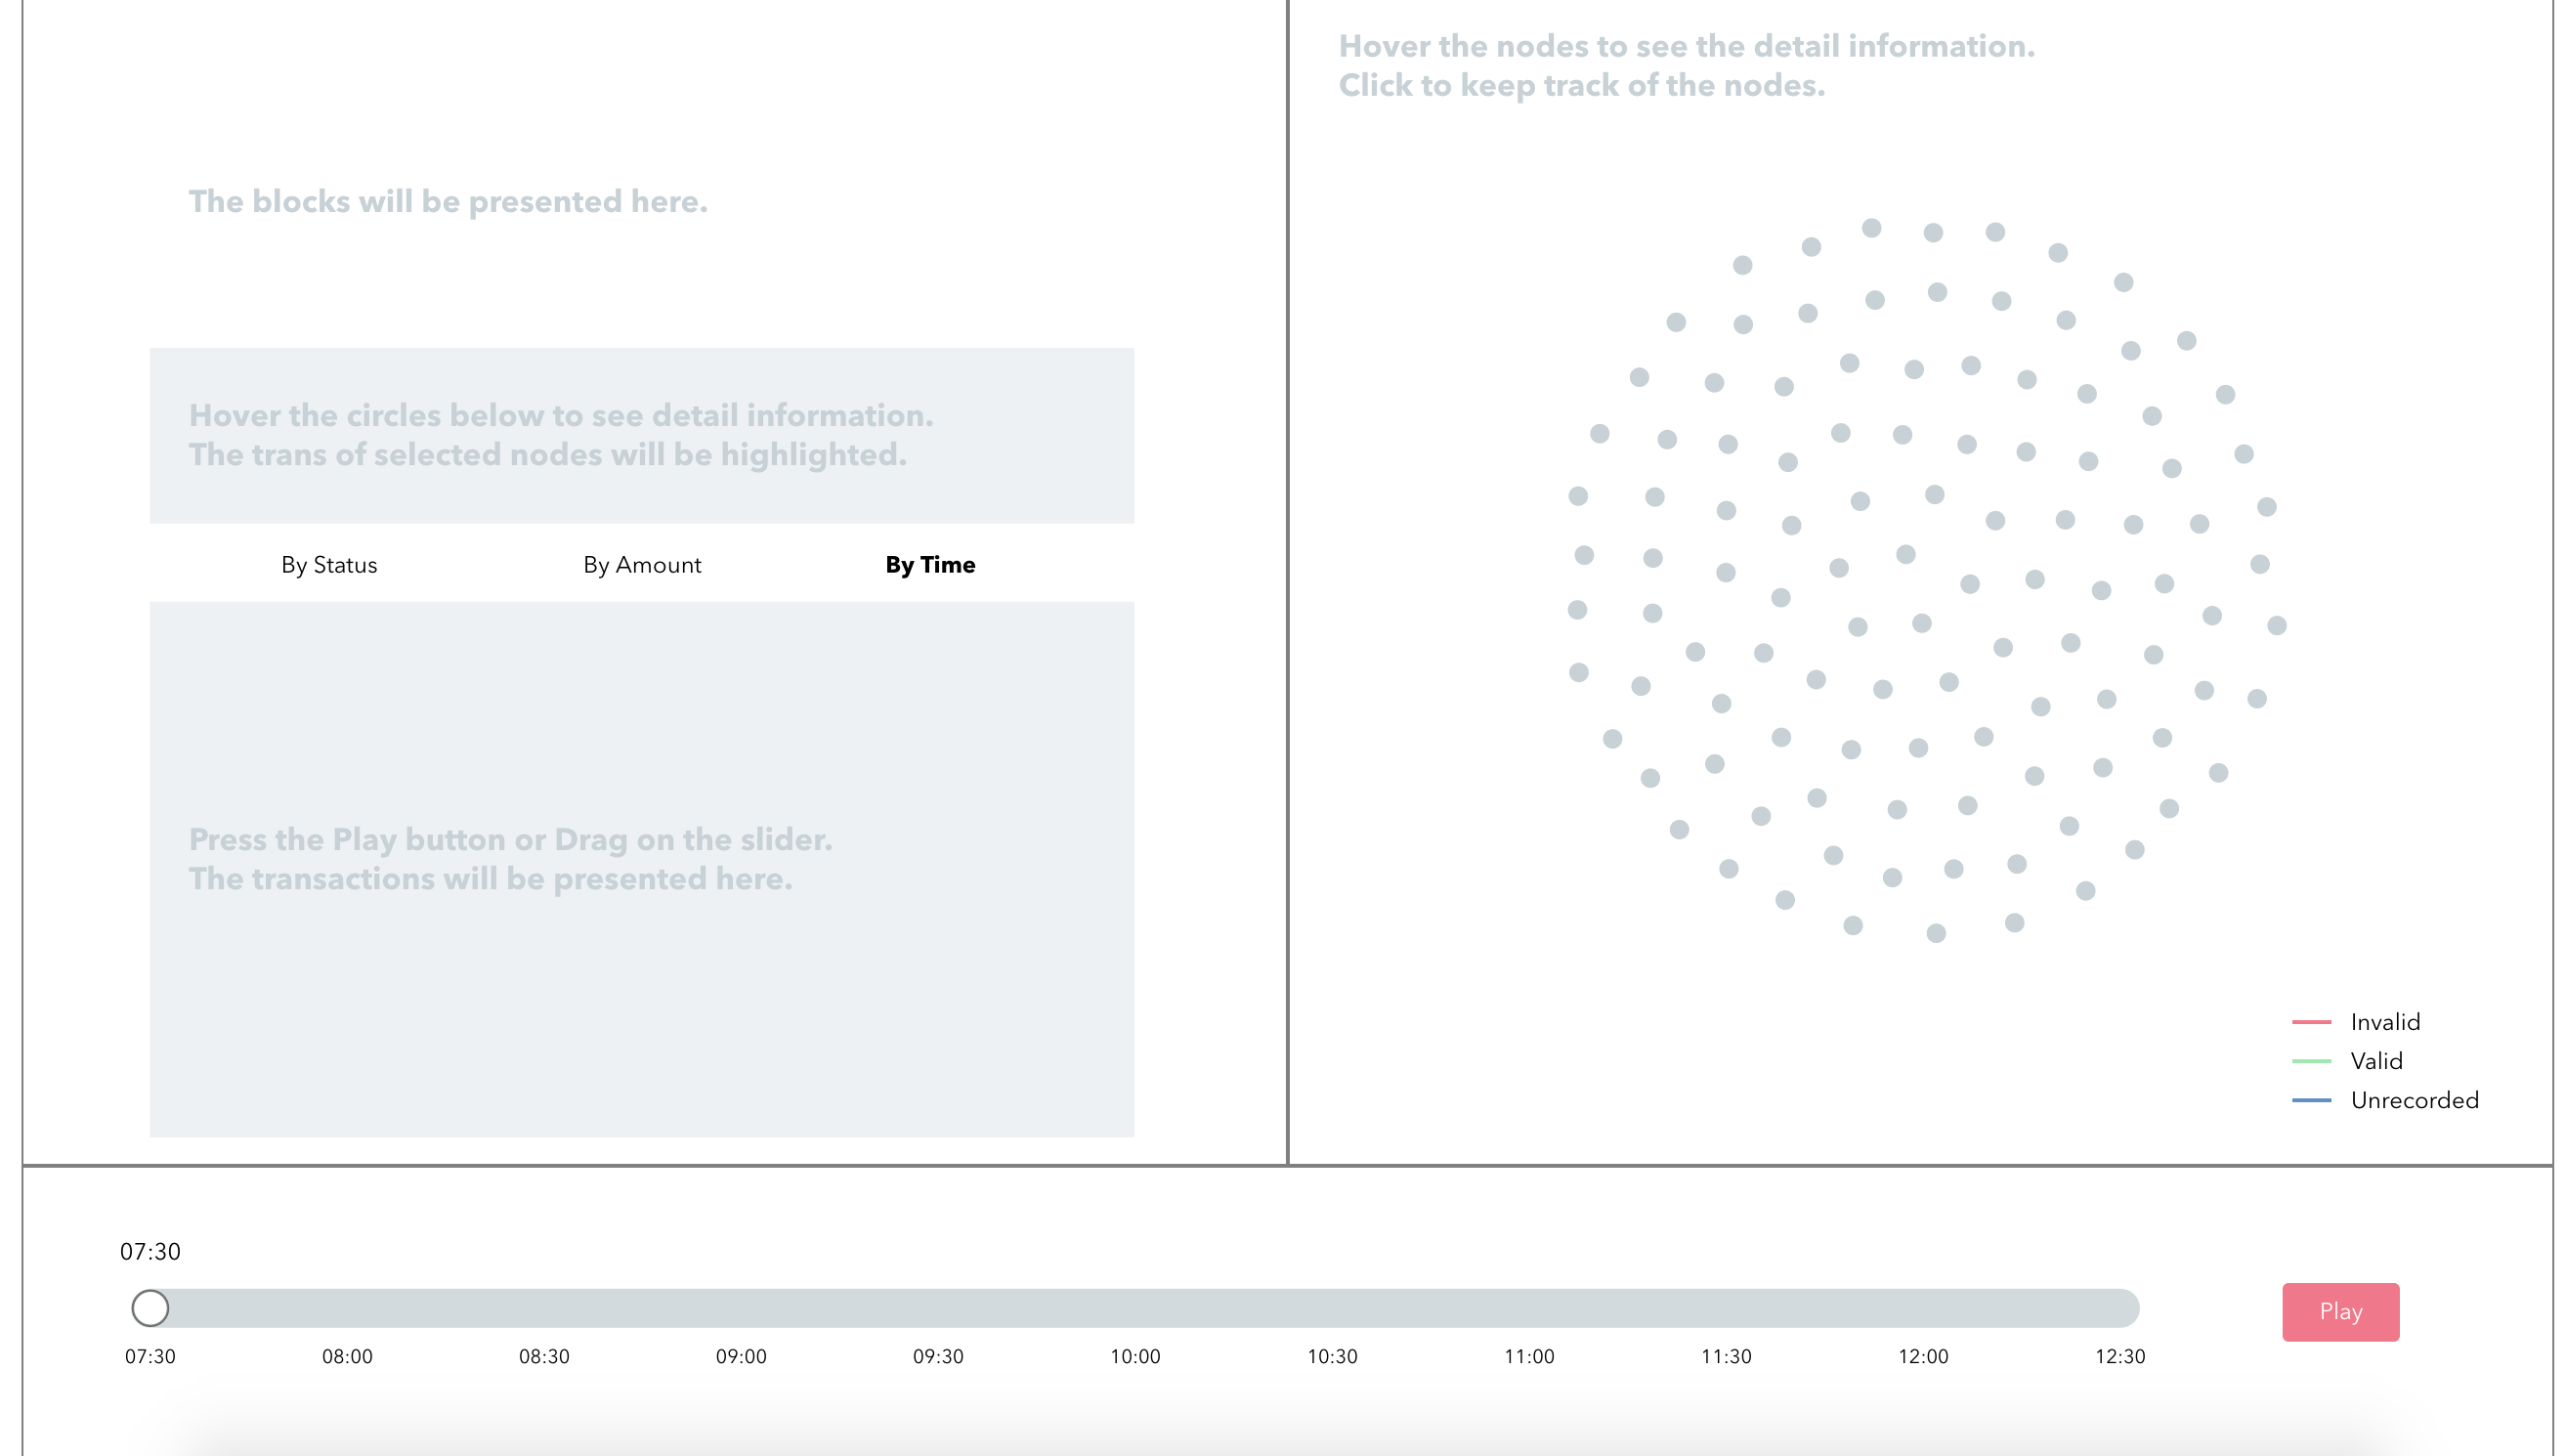
\includegraphics[width=\columnwidth]{overall_design_start.png}
		\caption{Initial state of bitcoin blockchain visualization}
		\label{fig:overall_design}
		\end{center}
	\end{figure}

Figure 3 is the state of bitcoin blockchain visualization at some time point.
\begin{itemize}
    \item Time slider: the smallest time interval is 5 minutes.
    \item Right panel: the color of the nodes demonstrates if it is active at the time
    \begin{itemize}
        \item grey: inactive, not involved in any transactions
        \item orange: active, involved in transactions
    \end{itemize}
    The links connect to the nodes that are related to transactions and their thickness demonstrate the transaction amount. The color of the links demonstrates the transaction status
    \begin{itemize}
        \item red: confirmed to be invalid transaction and should not been recorded in any block
        \item green: confirmed to be valid transaction and has been recorded in the latest block
        \item blue: unconfirmed and unrecorded in any block yet
    \end{itemize}
    \item Left panel's upper layer: the blocks in blockchain
    \begin{itemize}
        \item block\#: its rank in the blockchain by the time it is generated
        \item size: number of transactions recorded in this block
        \item color: dark grey is the color at the time point a block is generated. It will stay light grey after that.
    \end{itemize}
    \item Left panel's middle layer: hover the circles below and detail information of selected transaction will show up here. The transaction of selected nodes will also be highlighted in the right panel.
    \item Left panel's lower layer: circles represent transactions happening at this time point. The size of the circles demonstrates the transaction amount. The color of the circles demonstrates the status of the transactions.
    \begin{itemize}
        \item red: confirmed to be invalid transaction and should not been recorded in any block
        \item green: confirmed to be valid transaction and has been recorded in the latest block
        \item blue: unconfirmed and unrecorded in any block yet
    \end{itemize}
    you can also choose to sort or group the circles with the buttons that offered.
    \begin{itemize}
        \item By Status: circles will be grouped by status in order of red(invalid), blue(unrecorded) and green(valid).
        \item By Amount: circles will be sorted by amount in order of small to large.
        \item By Time: circles will be sorted by amount In chronological order. 
    \end{itemize}
\end{itemize}

\begin{figure}[!hbt]
		\begin{center}
		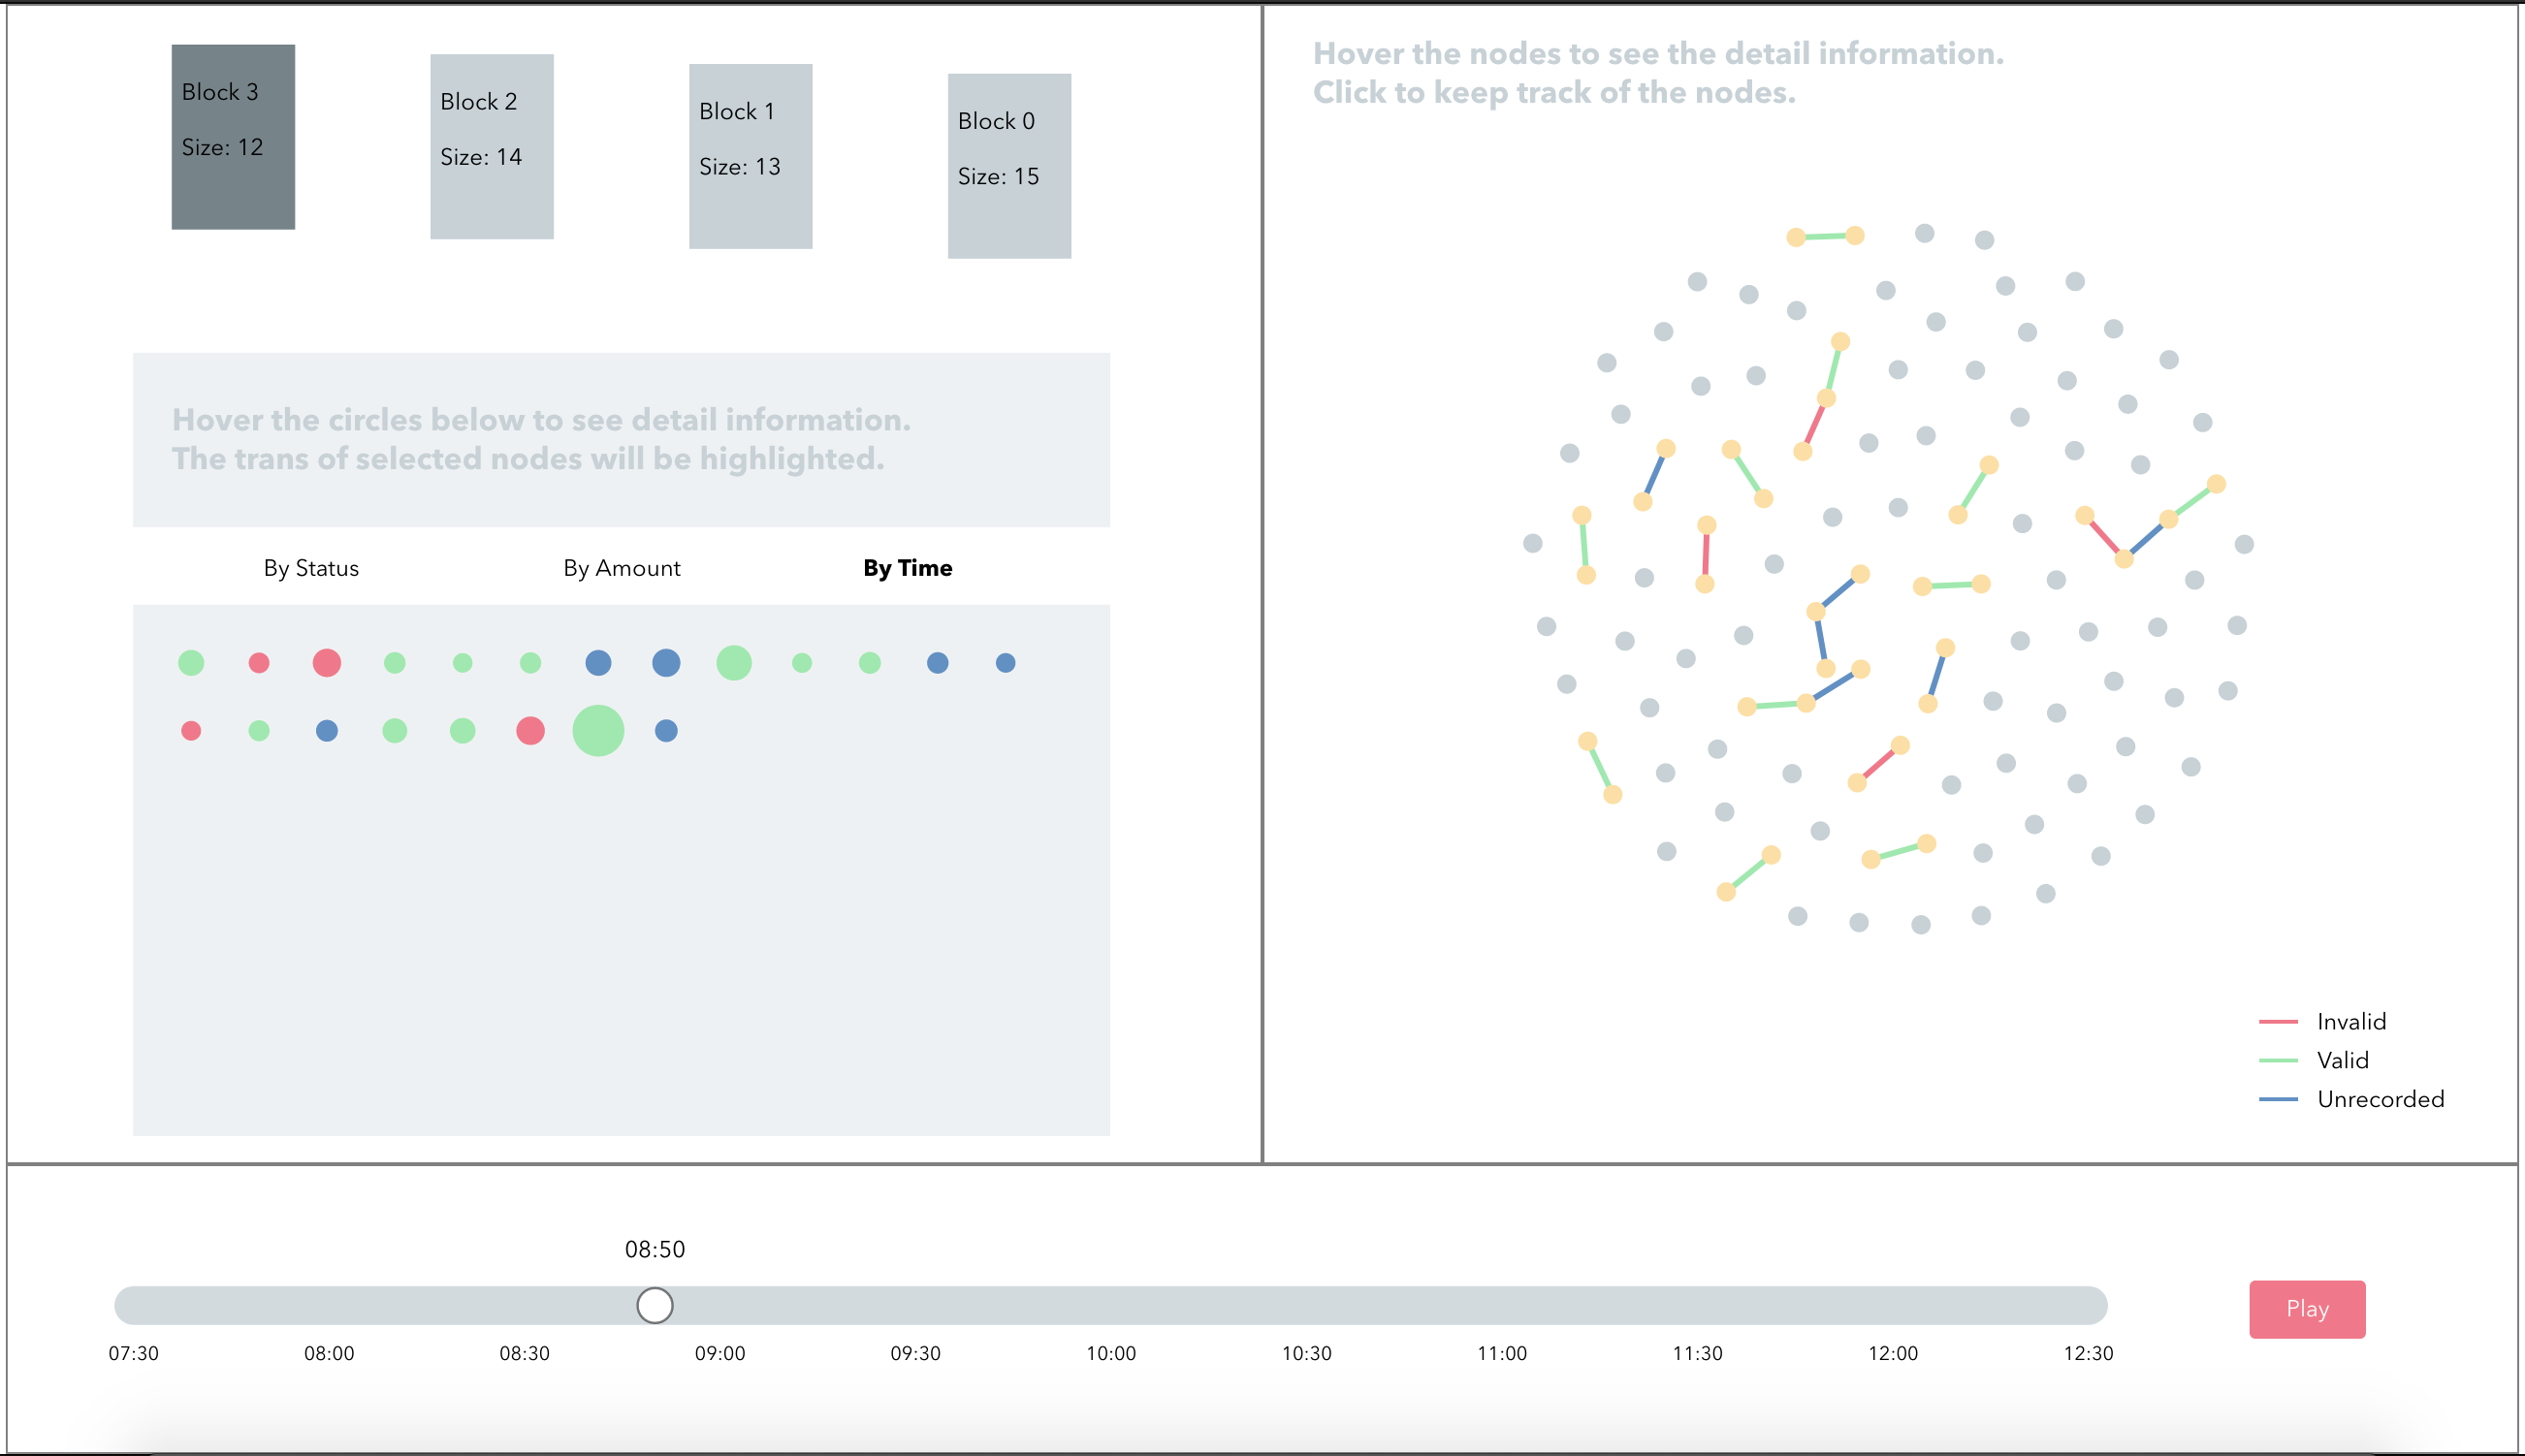
\includegraphics[width=\columnwidth]{overall_design.png}
		\caption{no-real time monitoring of bitcoin blockchain}
		\label{fig:overall_design}
		\end{center}
	\end{figure}

\section{Key intuitions behind our proposed design}
\subsection{Blockchain Demo}
We found an implementation of blockchain in JavaScript(Figure 4). Using this implementation as a base, we plan to mock and visualize the bitcoin blockchain by ourselves. Right now, the implementation required users to create new blocks and setup for different peers. We plan to change it to a format that take in a database and automatically go through all the steps. It?s in details but the data size is small, and it cannot offer users a board view of what transactions are happening behind the blockchain.

\begin{figure}[!hbt]
		\begin{center}
		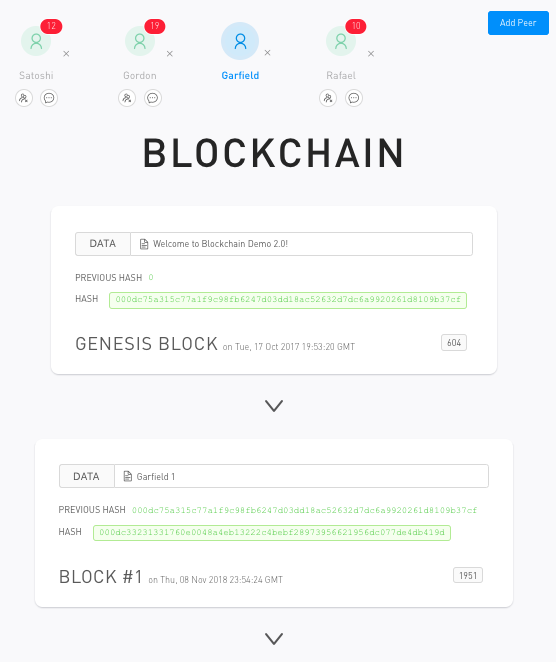
\includegraphics[width=\columnwidth]{blockchaindemo.png}
		\caption{Blockchain Demo, Link: \href{https://blockchaindemo.io}{https://blockchaindemo.io}}
		\label{fig:demo}
		\end{center}
	\end{figure}

\subsection{Ethereum blockchain visualization}
We found another live application for bitcoin that is implemented in Javascript(Figure 5). It?s nice visualization but the data size is big and the information is not in details. It offers users a board view of the transactions and blockchain, but give users little information inside each block.
\begin{figure}[!hbt]
		\begin{center}
		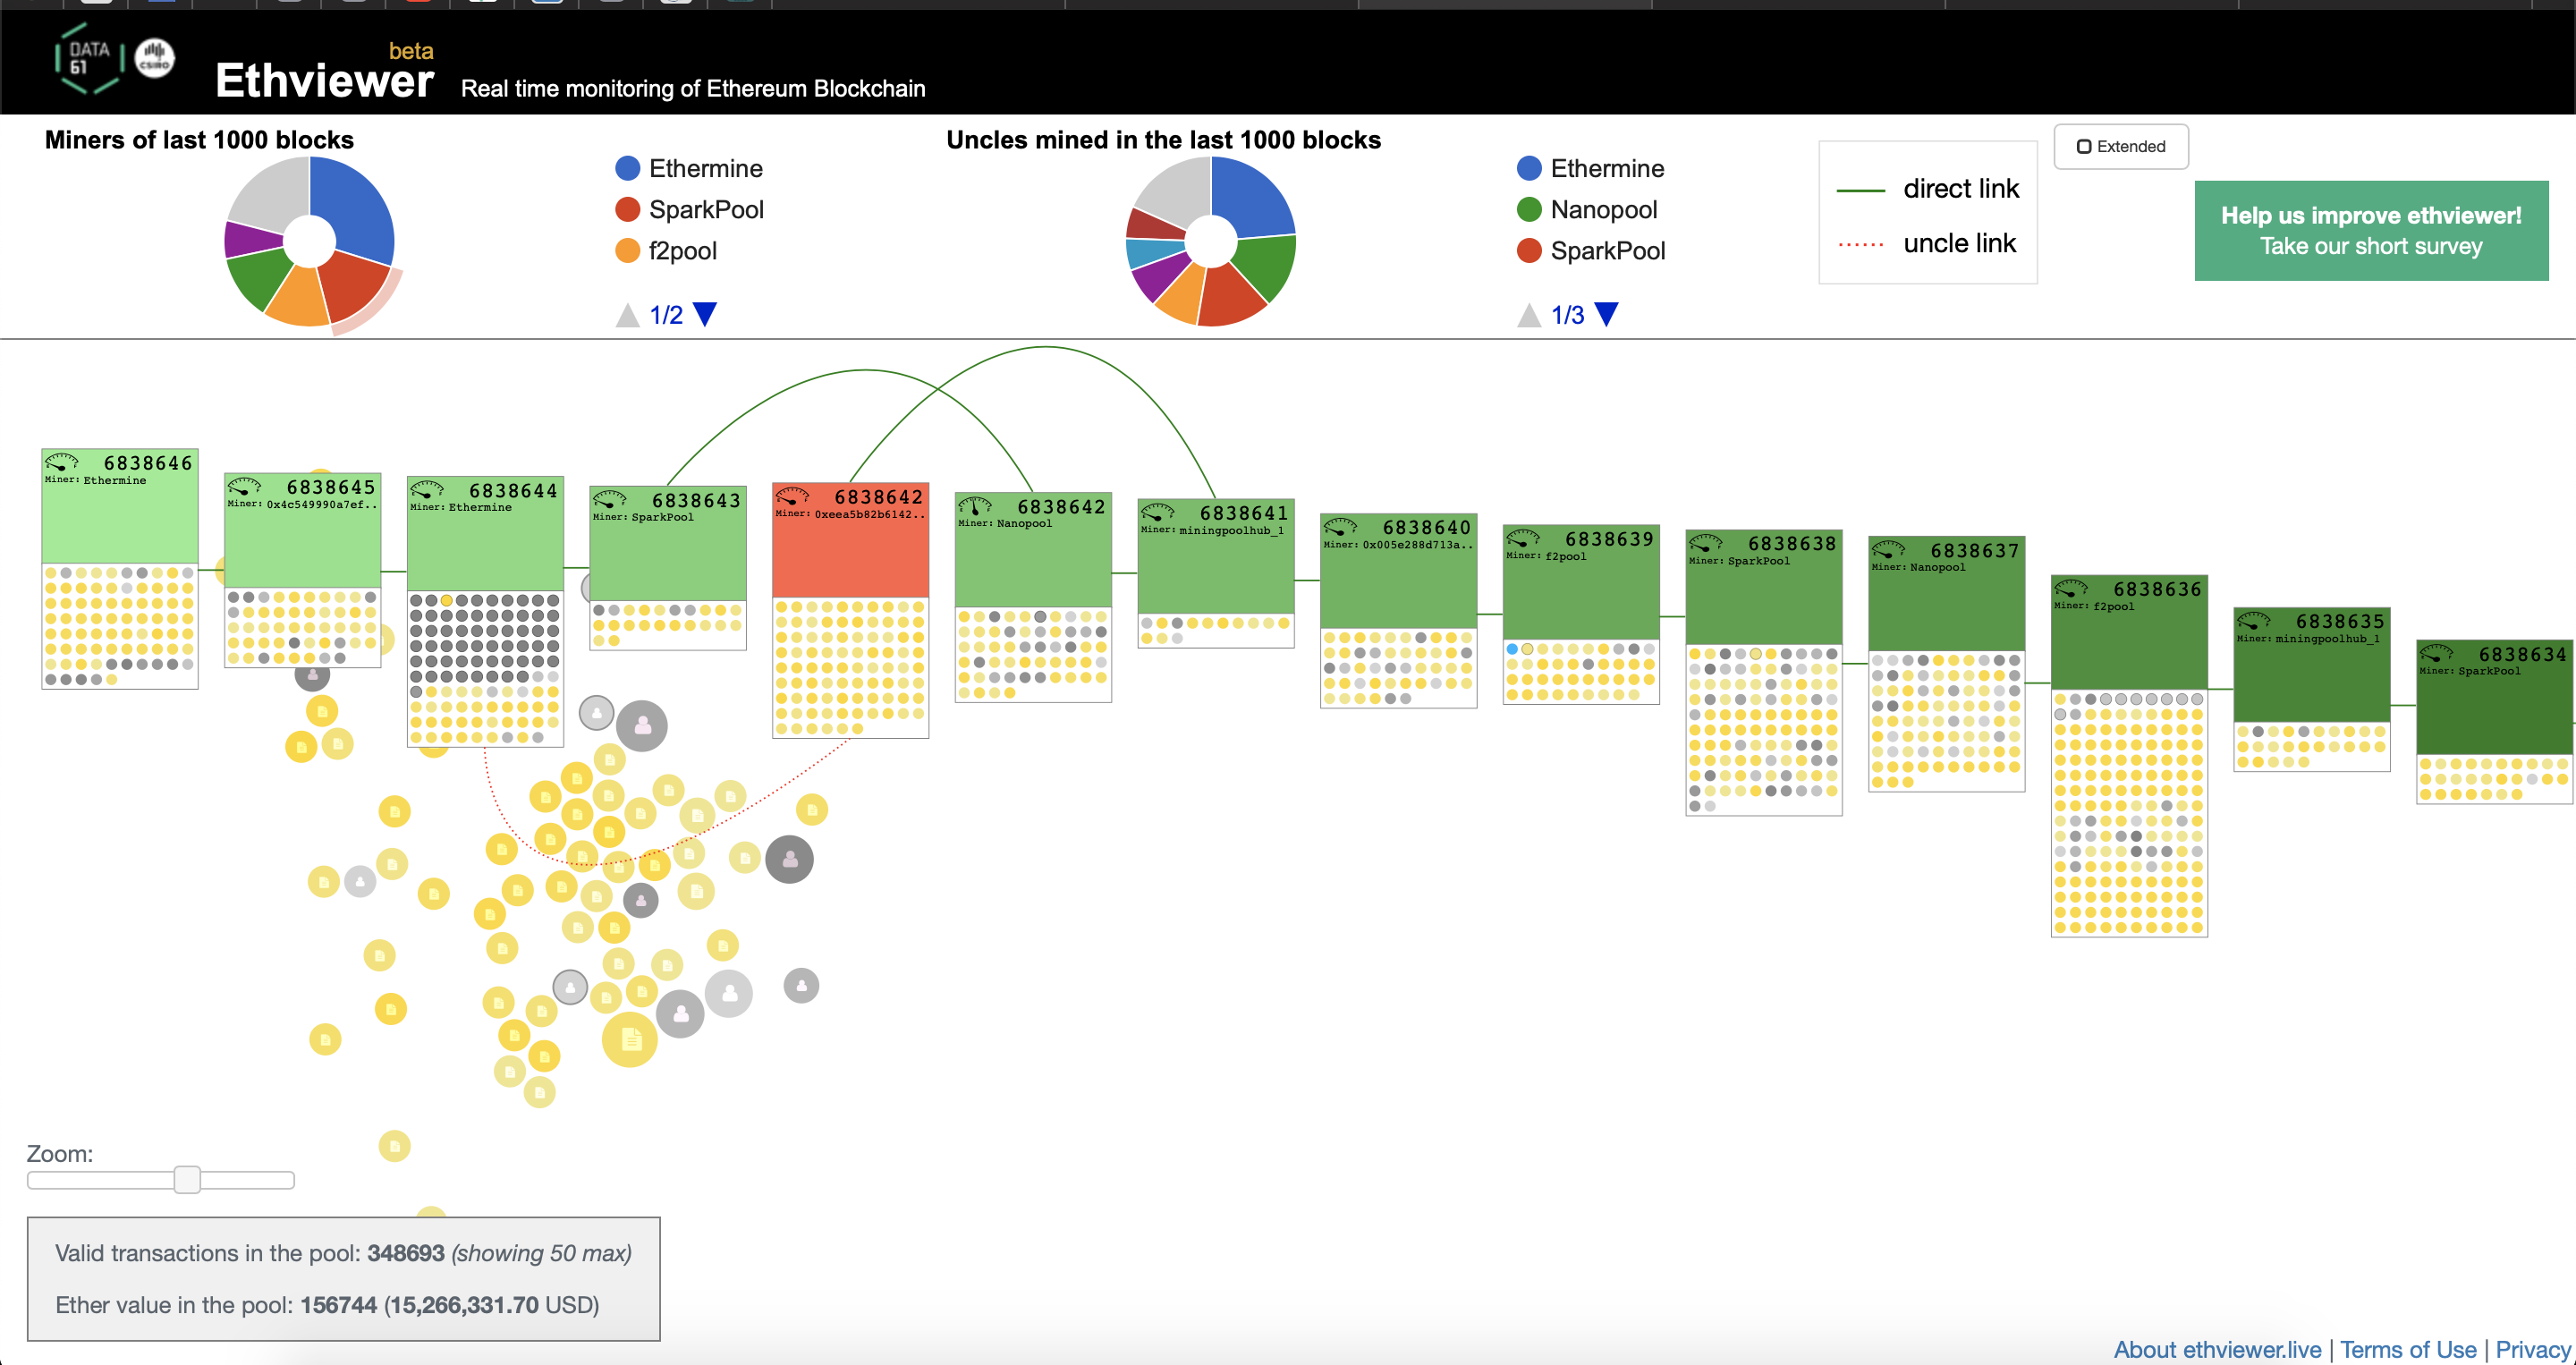
\includegraphics[width=\columnwidth]{ethereum.png}
		\caption{Ethereum blockchain visualization, Link: \href{http://www.ethviewer.live}{http://www.ethviewer.live}}
		\label{fig:Ethereum blockchain visualization}
		\end{center}
	\end{figure}

\section{Key benefits of our proposed design}

\section{Details of our design}
\subsection{Transactions}
Figure 6 is a live updating graph of addresses and bitcoin transactions between nodes.
\begin{figure}[!hbt]
		\begin{center}
		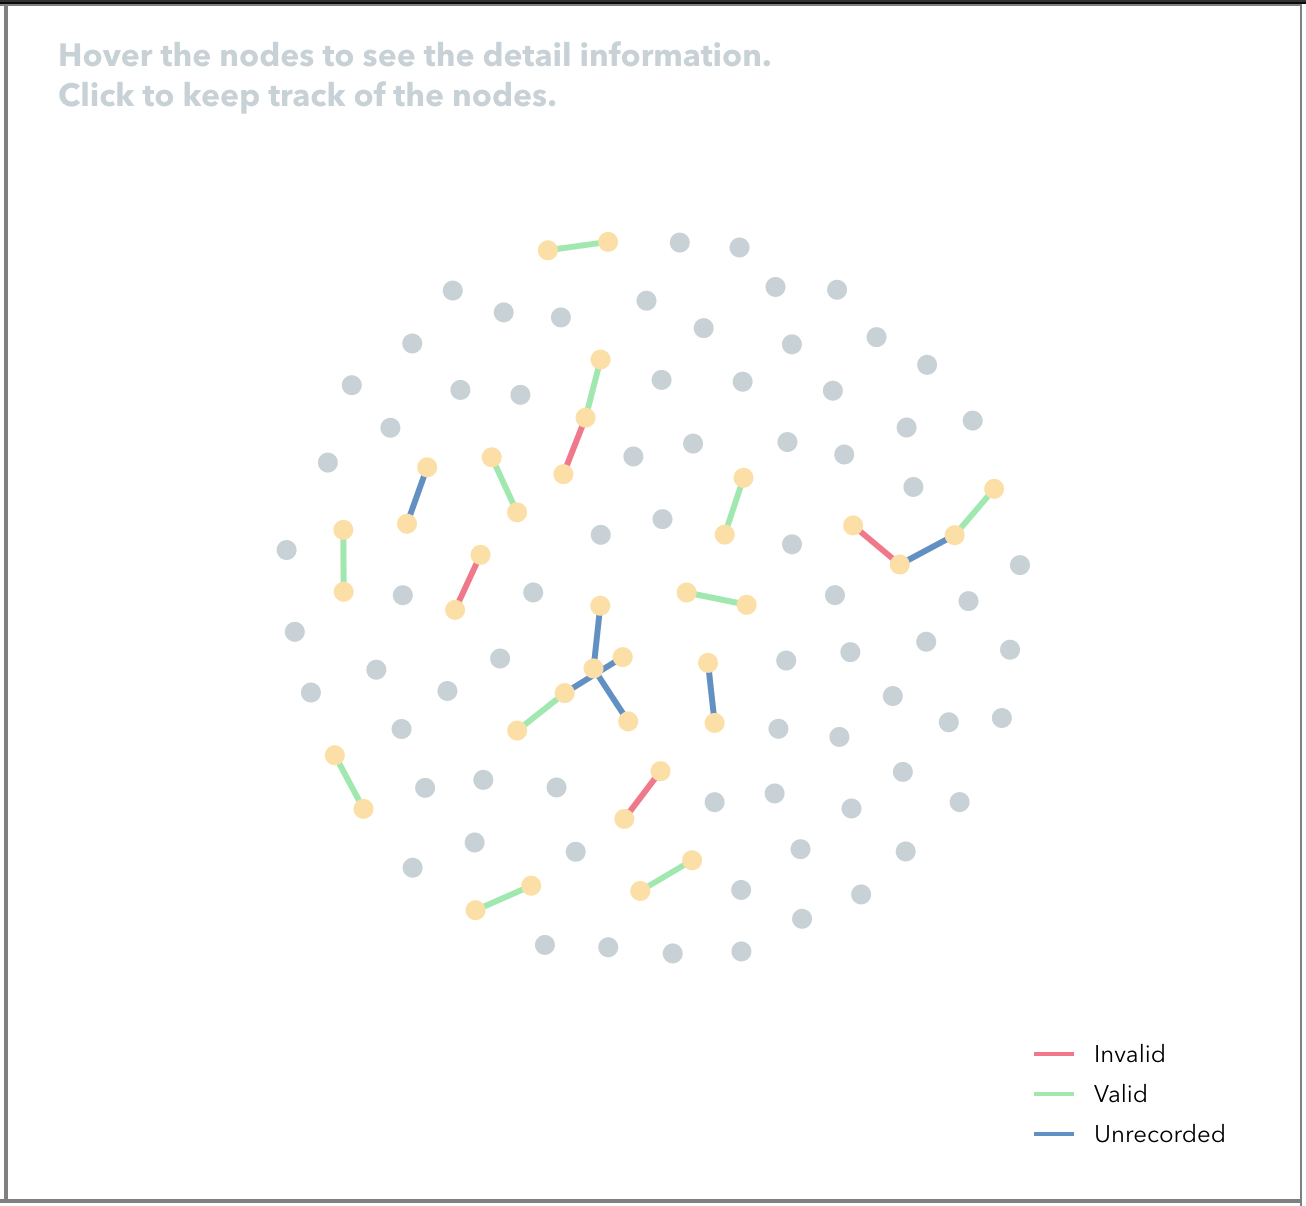
\includegraphics[width=\columnwidth]{transactions.png}
		\caption{bitcoin transactions}
		\label{fig:overall_design}
		\end{center}
	\end{figure}

Figure 7 shows detail information of the node when you hover it.
\begin{itemize}
    \item Address: public bitcoin address, identifiers which you use to send bitcoins to another person
    \item Hash: the hash of a public key, to shorten it.
    \item Nickname: we add this name to easily represent nodes
    \item Balance: we add this balance to show how many bitcoins one address owns at present, so the results of transactions can be visible.
\end{itemize}
\begin{figure}[!hbt]
		\begin{center}
		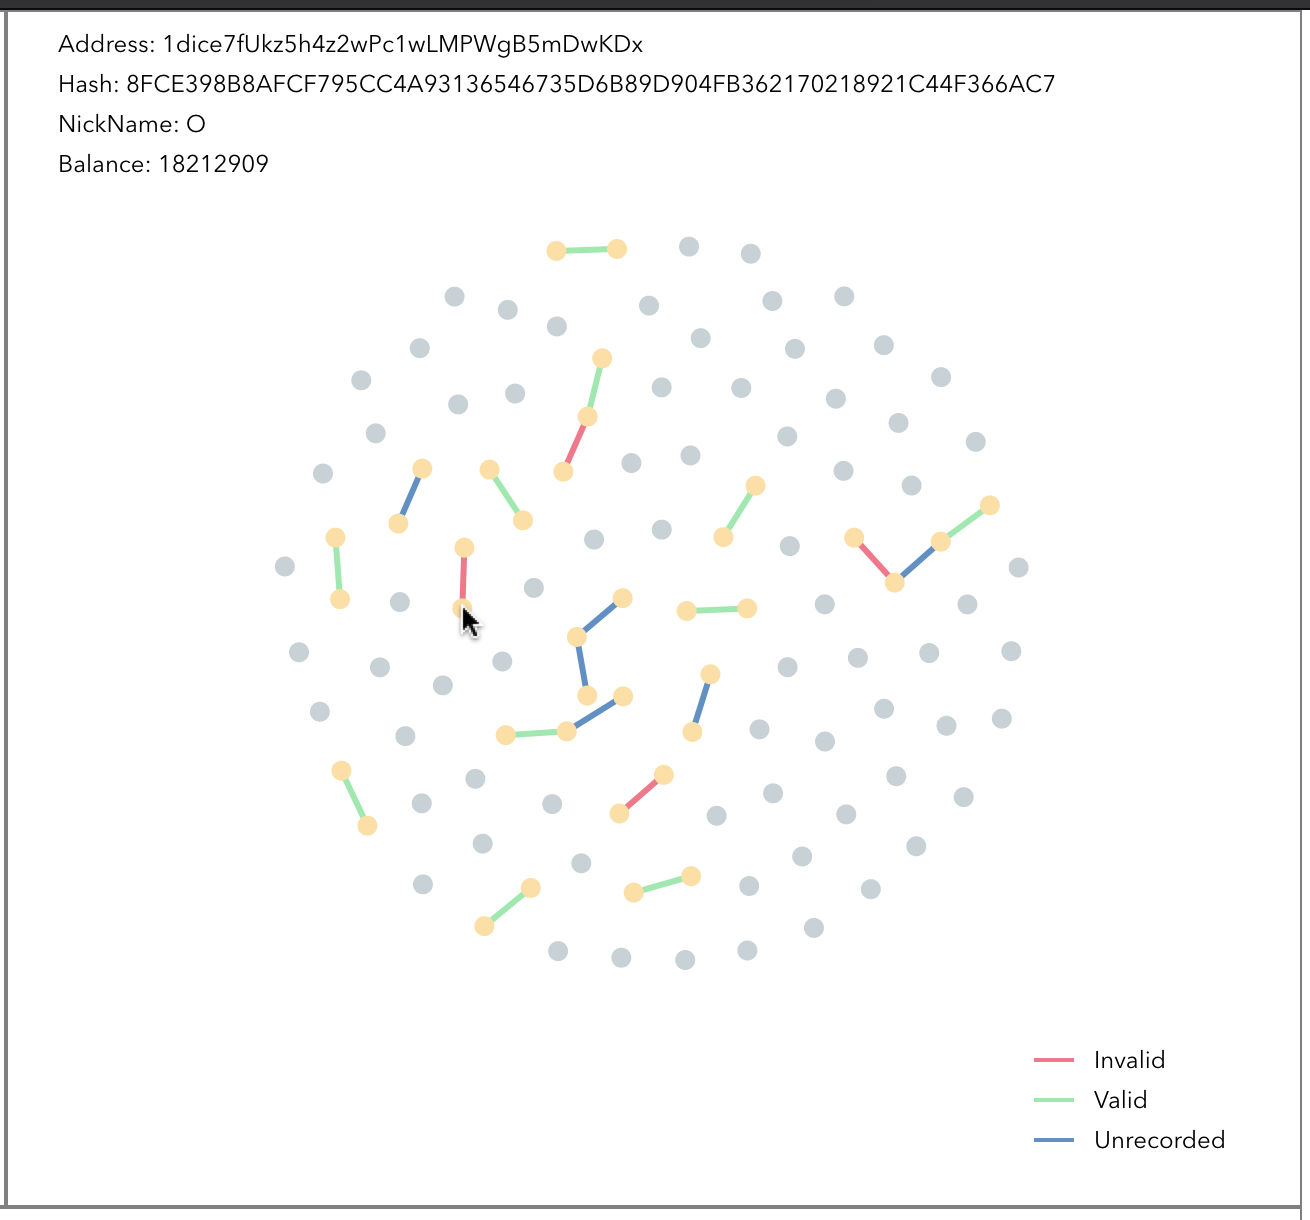
\includegraphics[width=\columnwidth]{transaction_hover.png}
		\caption{Hover the nodes to see the detail information}
		\label{fig:transaction_hover}
		\end{center}
	\end{figure}

\subsection{Blocks}
Figure 8 is a live updating left panel of bitcoin transactions between nodes.
\begin{figure}[!hbt]
		\begin{center}
		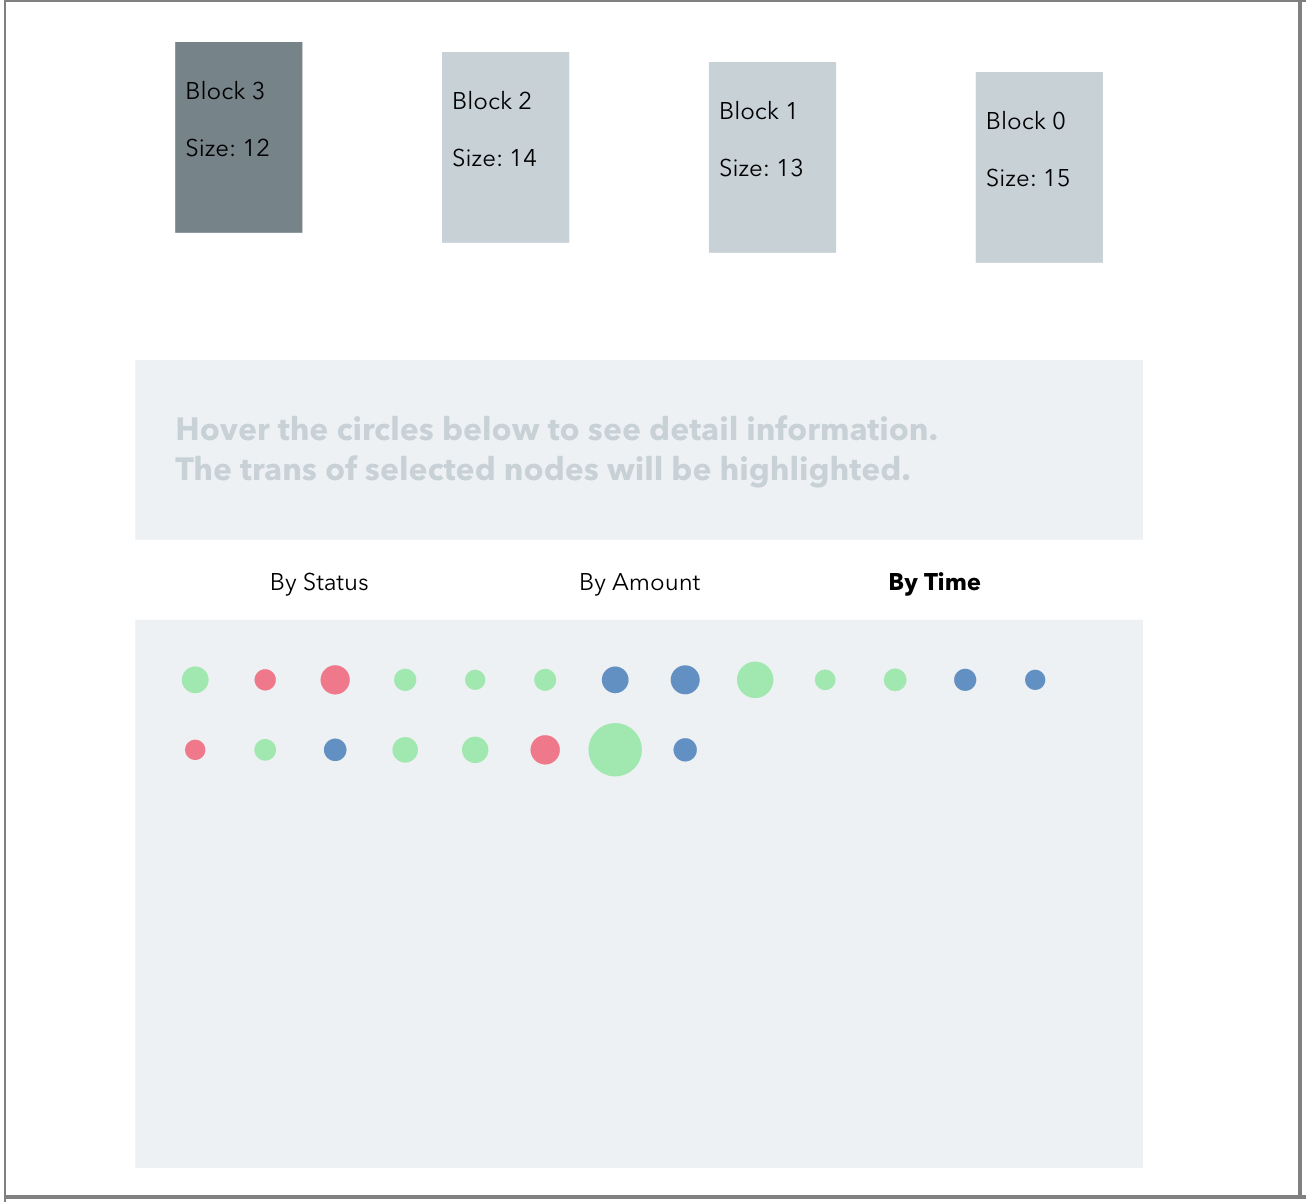
\includegraphics[width=\columnwidth]{blocks.png}
		\caption{bitcoin transactions}
		\label{fig:blocks}
		\end{center}
	\end{figure}
	
Figure 9 shows detail information of the circles below when you hover it.
\begin{itemize}
    \item Status: VALID (green), INVALID (red) and UNRECORDED (blue)
    \item Trans: from Nickname to Nickname with amount of bitcoin transacted
    \item Time: the time point when this transaction is generated
    \item Block: the \# of block to which this transaction belongs
\end{itemize}
\begin{figure}[!hbt]
		\begin{center}
		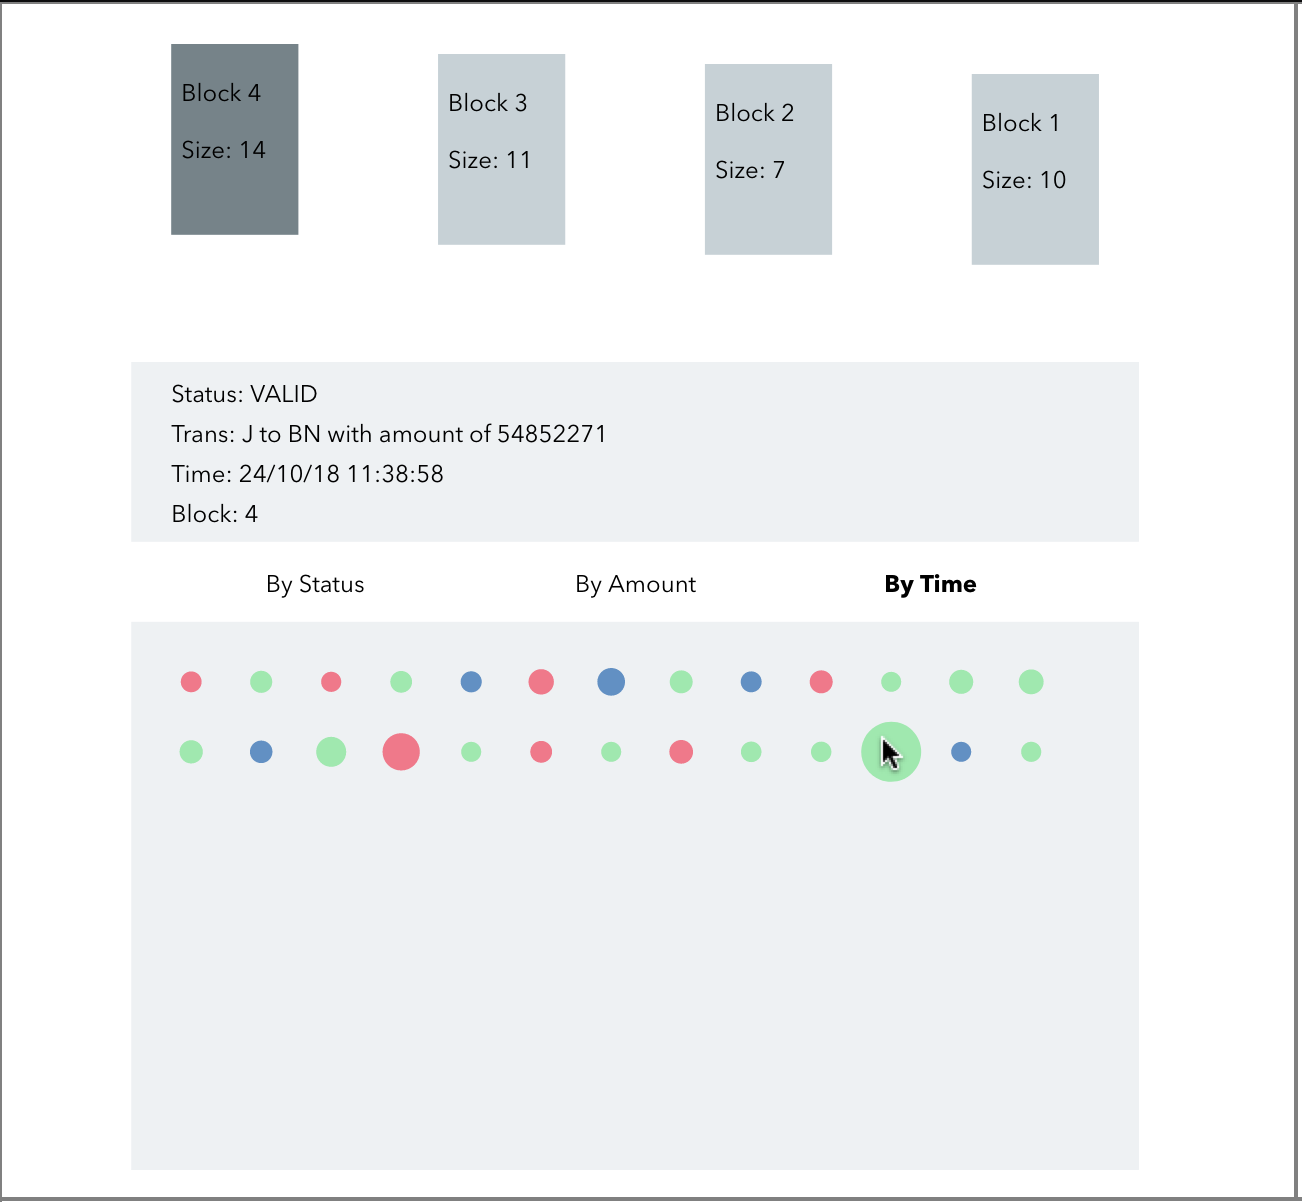
\includegraphics[width=\columnwidth]{block_hover.png}
		\caption{Hove the circle to see the detail information}
		\label{fig:block_hover}
		\end{center}
	\end{figure}

\subsection{Interaction of left and right panels}
Figure 10 shows the interaction of left and right panels. The nodes you select on the right panel will be highlighted on the right panel. All transactions related to the selected nodes will be highlighted on both left and right panels.
\begin{figure}[!hbt]
		\begin{center}
		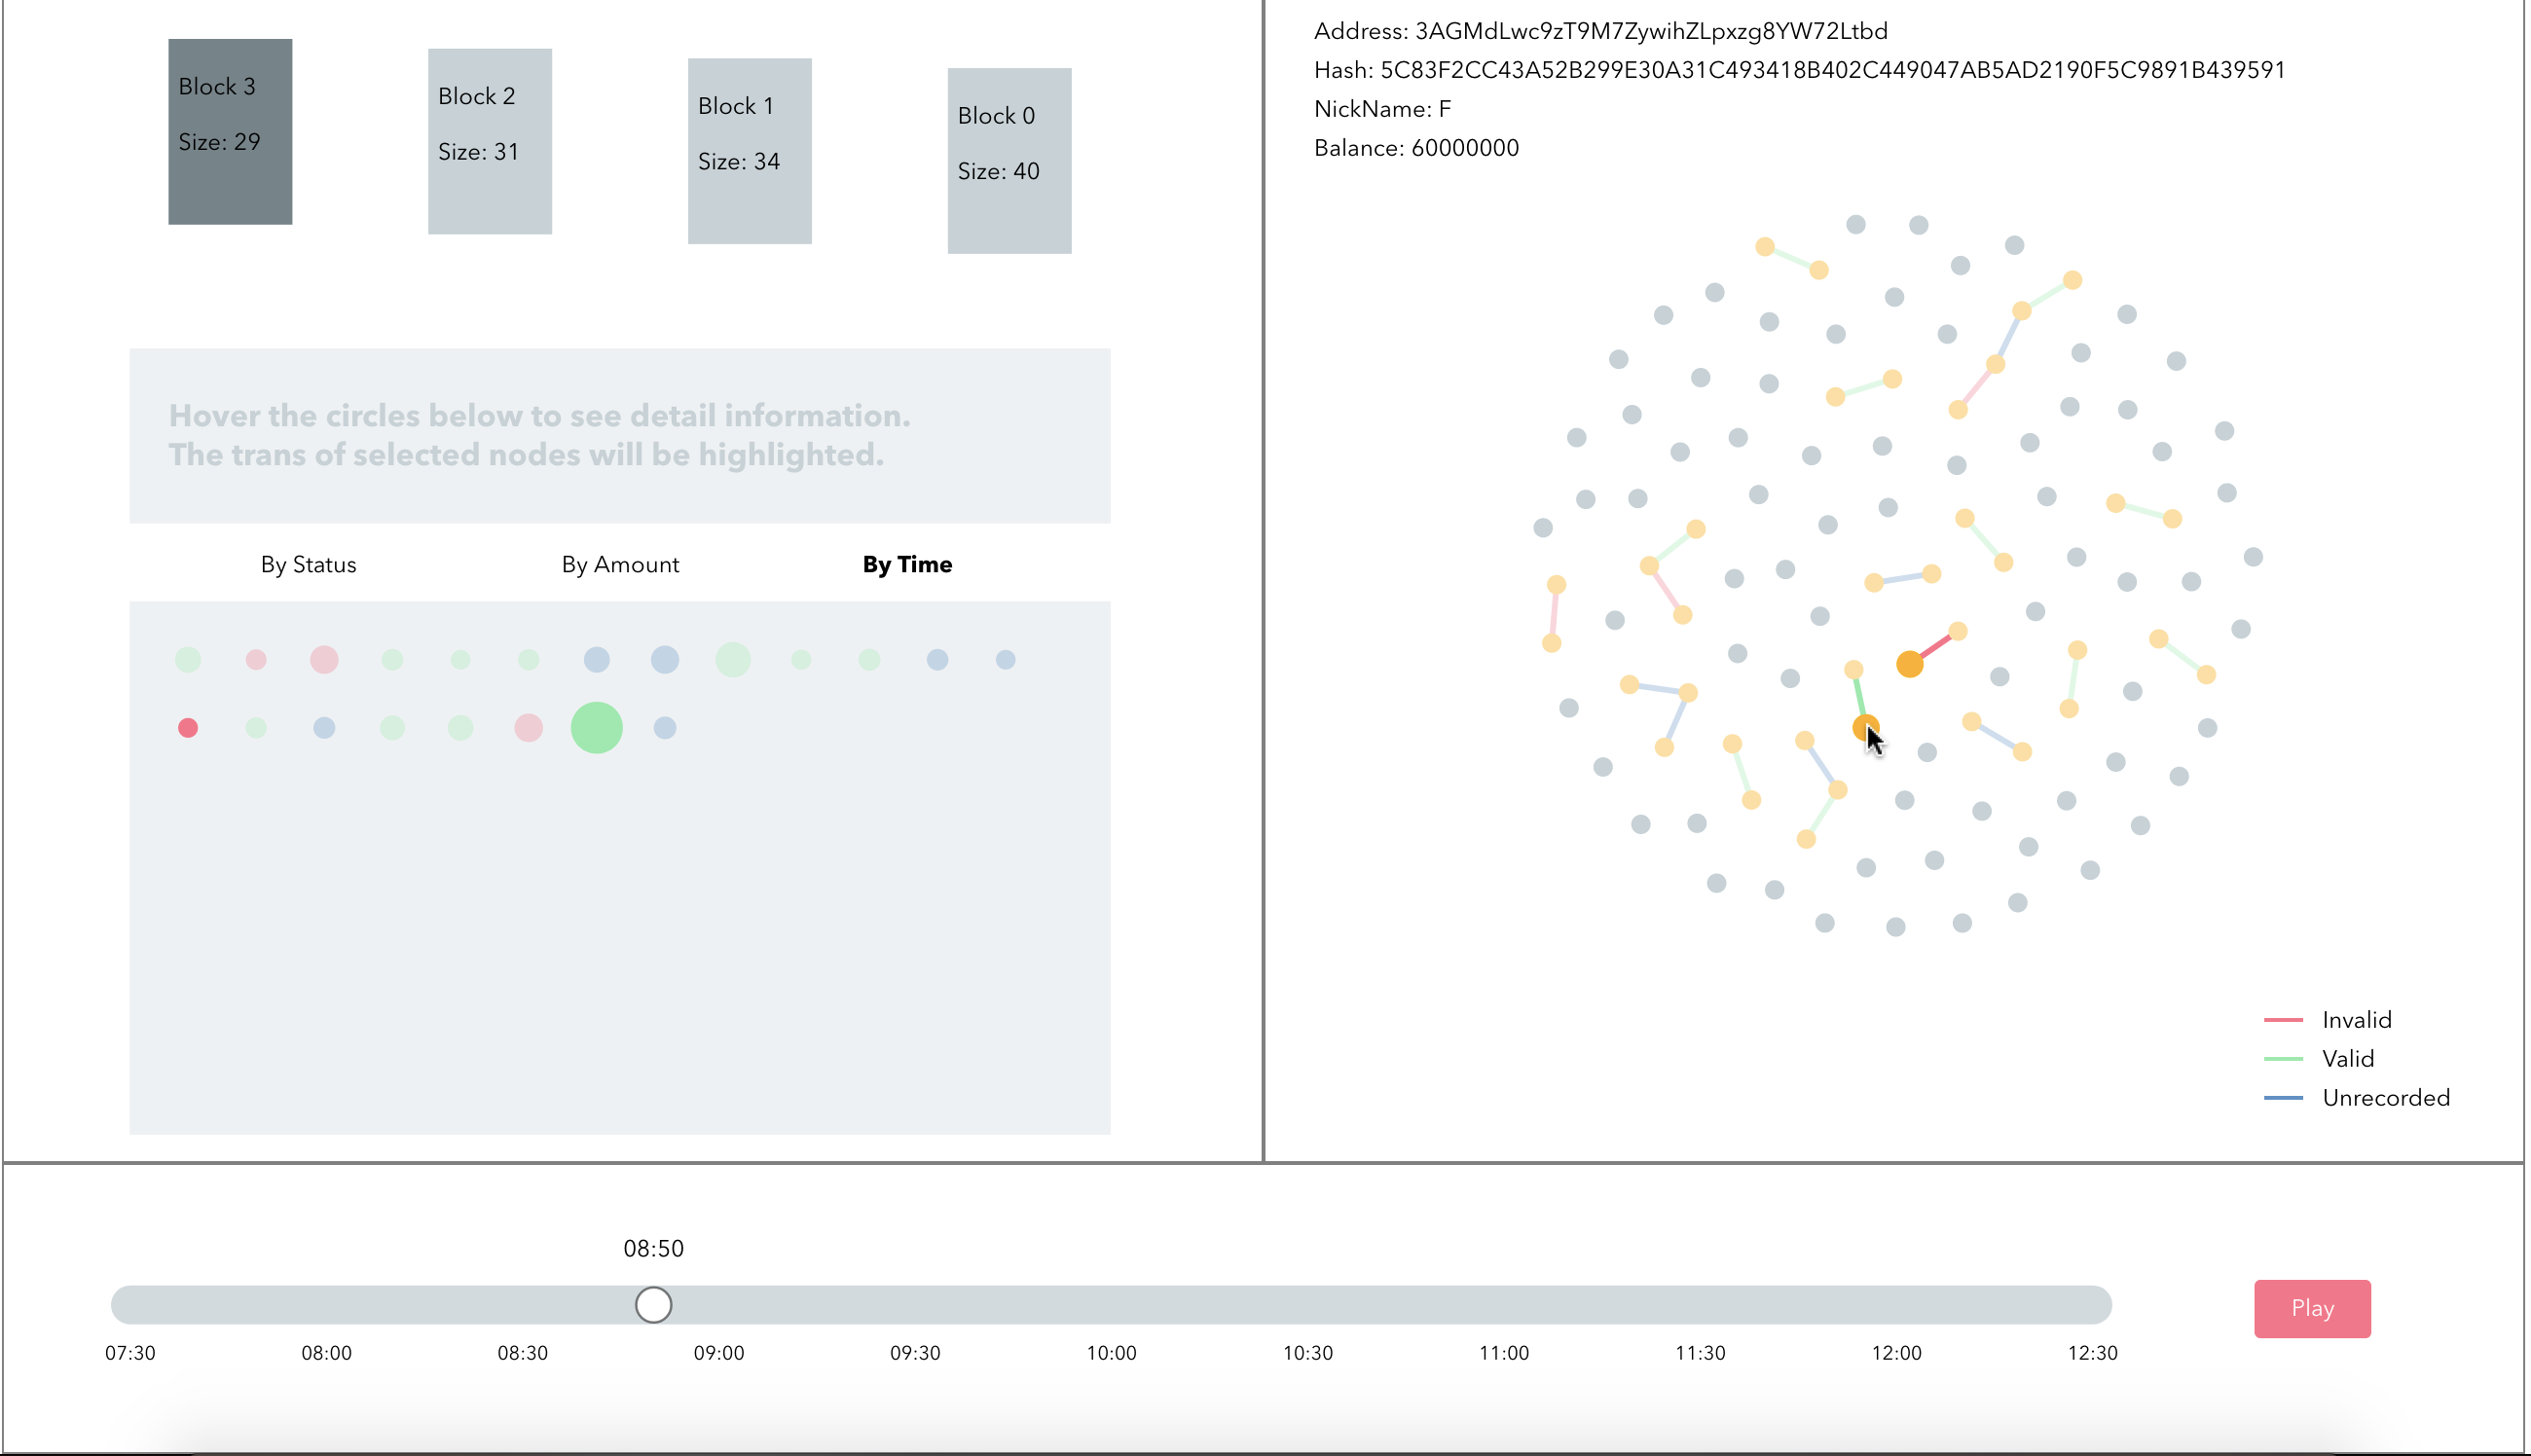
\includegraphics[width=\columnwidth]{clicknodes.png}
		\caption{Interaction of left and right panels}
		\label{fig:clicknodes}
		\end{center}
	\end{figure}

\section{Contributions}
Zhiyi ; Ruolan.
\section{Conclusions}

\section{Future Directions}
Despite Bitcoin?s potential, blockchain protocols face a significant scalability barrier. The maximum rate at which these systems can process transactions is capped by the choice of two parameters: block size and block interval.
\begin{itemize}
    \item Increasing block size improves throughput, but the resulting bigger blocks take longer to propagate in the network.
    \item Reducing the block interval reduces latency, but leads to instability where the system is in disagreement and the blockchain is subject to reorganization.
\end{itemize}
We want to learn and try to implement Bitcoin-NG (Next Generation), a new blockchain protocol designed to scale, presented in \text{Bitcoin-NG: A Scalable Blockchain Protocol}. It is a Byzantine fault tolerant blockchain protocol that is robust to extreme churn and shares the same trust model as Bitcoin. Finally, we want to compare the transaction frequency, consensus latency, fairness, mining power utilization, time to win and time to prune of Bitcoin and Bitcoin-NG at the same block frequency or block size to see if Bitcoin-NG can reduce latency and increase throughput, and whether it is possible to improve the scalability of blockchain protocols to the point where the consensus latency is limited solely by the network diameter and the throughput bottleneck lies only in node processing power.

\begin{thebibliography}{5}

	%Each item starts with a \bibitem{reference} command and the details thereafter.
	\bibitem{HOP96} % Transaction paper
	J.~Hagenauer, E.~Offer, and L.~Papke. Iterative decoding of binary block
	and convolutional codes. {\em IEEE Trans. Inform. Theory},
	vol.~42, no.~2, pp.~429?-445, Mar. 1996.

\end{thebibliography}

% Your document ends here!
\end{document}